% -------------------------------------------------------------------------------
% Establish page structure & font.
\documentclass[12pt]{report}

\usepackage[total={6.5in, 9in},
	left=1in,
	right=1in,
	top=1in,
	bottom=1in,]{geometry} % Page structure

\usepackage{graphicx} % Required for inserting images
\graphicspath{{../../.images}} % Any additional images I use (BCU logo, etc) are from here.

\usepackage[utf8]{inputenc} % UTF-8 encoding
\usepackage[T1]{fontenc} % T1 font
\usepackage{float}  % Allows for floats to be positioned using [H], which correctly
                    % positions them relative to their location within my LaTeX code.
\usepackage{subcaption}
\usepackage{csquotes}

% -------------------------------------------------------------------------------
% Declare biblatex with custom Harvard BCU styling for referencing.
\usepackage[
    useprefix=true,
    maxcitenames=3,
    maxbibnames=99,
    style=authoryear,
    dashed=false, 
    natbib=true,
    url=false,
    backend=biber
]{biblatex}

\usepackage[british]{babel}

% Additional styling options to ensure Harvard referencing format.
\renewbibmacro*{volume+number+eid}{
    \printfield{volume}
    \setunit*{\addnbspace}
    \printfield{number}
    \setunit{\addcomma\space}
    \printfield{eid}}
\DeclareFieldFormat[article]{number}{\mkbibparens{#1}}

\addbibresource{Proposal.bib}

% -------------------------------------------------------------------------------
% To prevent "Chapter N" display for each chapter
\usepackage[compact]{titlesec}
\usepackage{wasysym}
\usepackage{import}

\titlespacing*{\chapter}{0pt}{-2cm}{0.5cm}
\titleformat{\chapter}[display]
{\normalfont\bfseries}{}{0pt}{\Huge}

% -------------------------------------------------------------------------------
% Custom macro to make an un-numbered footnote.

\newcommand\blfootnote[1]{
    \begingroup
    \renewcommand\thefootnote{}\footnote{#1}
    \addtocounter{footnote}{-1}
    \endgroup
}

% -------------------------------------------------------------------------------
% Fancy headers; used to show my name, BCU logo and current chapter for the page.
\usepackage{fancyhdr}
\usepackage{calc}
\pagestyle{fancy}

\setlength\headheight{37pt} % Set custom header height to fit the image.

\renewcommand{\chaptermark}[1]{%
    \markboth{#1}{}} % Include chapter name.


% Lewis Higgins - ID 22133848           [BCU LOGO]                [CHAPTER NAME]
\lhead{Lewis Higgins - ID 22133848~~~~~~~~~~~~~~~
\includegraphics[width=1.75cm]{BCU}}
\fancyhead[R]{\leftmark}

% ------------------------------------------------------------------------------
% Used to add PDF hyperlinks for figures and the contents page.

\usepackage{hyperref}

\hypersetup{
    colorlinks=true,
    linkcolor=black,
    filecolor=magenta,
    urlcolor=blue,
    citecolor=black,
}

% ------------------------------------------------------------------------------
\usepackage{xcolor} 
\usepackage{colortbl}
\usepackage{longtable}
\usepackage{amssymb}
% ------------------------------------------------------------------------------
\usepackage{tcolorbox}
\newcommand{\para}{\vspace{7pt}\noindent}
% -------------------------------------------------------------------------------

\title{Project Proposal}
\author{Lewis Higgins - Student ID 22133848}
\date{March 2025}

% -------------------------------------------------------------------------------

\begin{document}


\makeatletter
\begin{titlepage}
    \begin{center}
        
\includegraphics[width=0.7\linewidth]{BCU}\\[4ex]
        {\huge \bfseries CMP6228 - Deep Learning Project}\\[2ex]
        {\large \bfseries  \@title}\\[50ex]
        {\@author}\\[2ex]
        {CMP6228 - Deep Neural Networks}\\[2ex]
        {Module Coordinator: Khalid Ismail}\\[2ex]
        {Word count excluding figures, references and appendices: XXXX / 1500}\\[10ex]
    \end{center}
\end{titlepage}
\makeatother
\thispagestyle{empty}
\newpage

% Page counter trick so that the contents page doesn't increment it.
\setcounter{page}{0}

\tableofcontents
\thispagestyle{empty}

\chapter*{Introduction}
\addcontentsline{toc}{chapter}{Introduction}

In this report, a novel solution is proposed to address a significant data science problem in the medical field, in the form of 
a deep neural network to accurately identify the presence of pneumonia from an image of a chest X-ray. To do so, this neural network 
will be trained on a publicly available dataset that has been previously seen across many publications, and advanced techniques 
for the model will be discussed.

\para This proposal will specifically cover the motivation behind this project before exploring related literature and previous works 
in great depth. To conclude, an optimal model will be proposed based on the knowledge extracted from these related works. 

% ! Weak. Come back to this probably at the very end.


\chapter{Motivation and objectives}

\section{Subject area}

Pneumonia is a lower respiratory tract infection (LRTI) commonly caused by viruses or bacteria wherein the alveoli of the lungs 
become clogged with pus and fluid, which can be life-threatening in people of any age, but especially in children and the elderly
\autocite{nhsPneumonia2017}. The World Health Organisation (WHO) state that pneumonia is the single largest infectious cause of death 
in children, killing 808,000 under the age of 5 in 2017 \autocite{whoPneumonia}. Even if pneumonia is survived during the initial infection,
\textcite{allinsonEarlyChildhoodLower2023} write that those who contract the condition as a child are 93\% more likely to die from respiratory
diseases later in life.

\para It is therefore imperative that recent technological advancements are leveraged for the quick diagnosis of the infection to allow swift 
treatment to avoid life-threatening consequences. 

\section{Dataset choice}
The chosen dataset is sourced from the Mendeley data repository \autocite{mendeleydataLargeDatasetLabeled}, uploaded and created by  
\textcite[p.1127]{kermanyIdentifyingMedicalDiagnoses2018} in their research of the applications of neural networks for medical diagnoses\footnote{Because their work was not only on pneumonia, the Mendeley ZIP file contains two separate datasets. This proposal is only for the "chest\_xray" dataset.}. 
The dataset contains 5,856 images of chest X-ray scans of children taken from the University of California San Diego in America as well as the
Guangzhou Women and Children's Medical Center in China, and is 1.18GB in size. There are only two classes of images: those with 
pneumonia and those without, as depicted by Figures \ref{fig:SampleNORMAL} and \ref{fig:SamplePNEUMONIA}.

\begin{figure}[H]
    \centering
    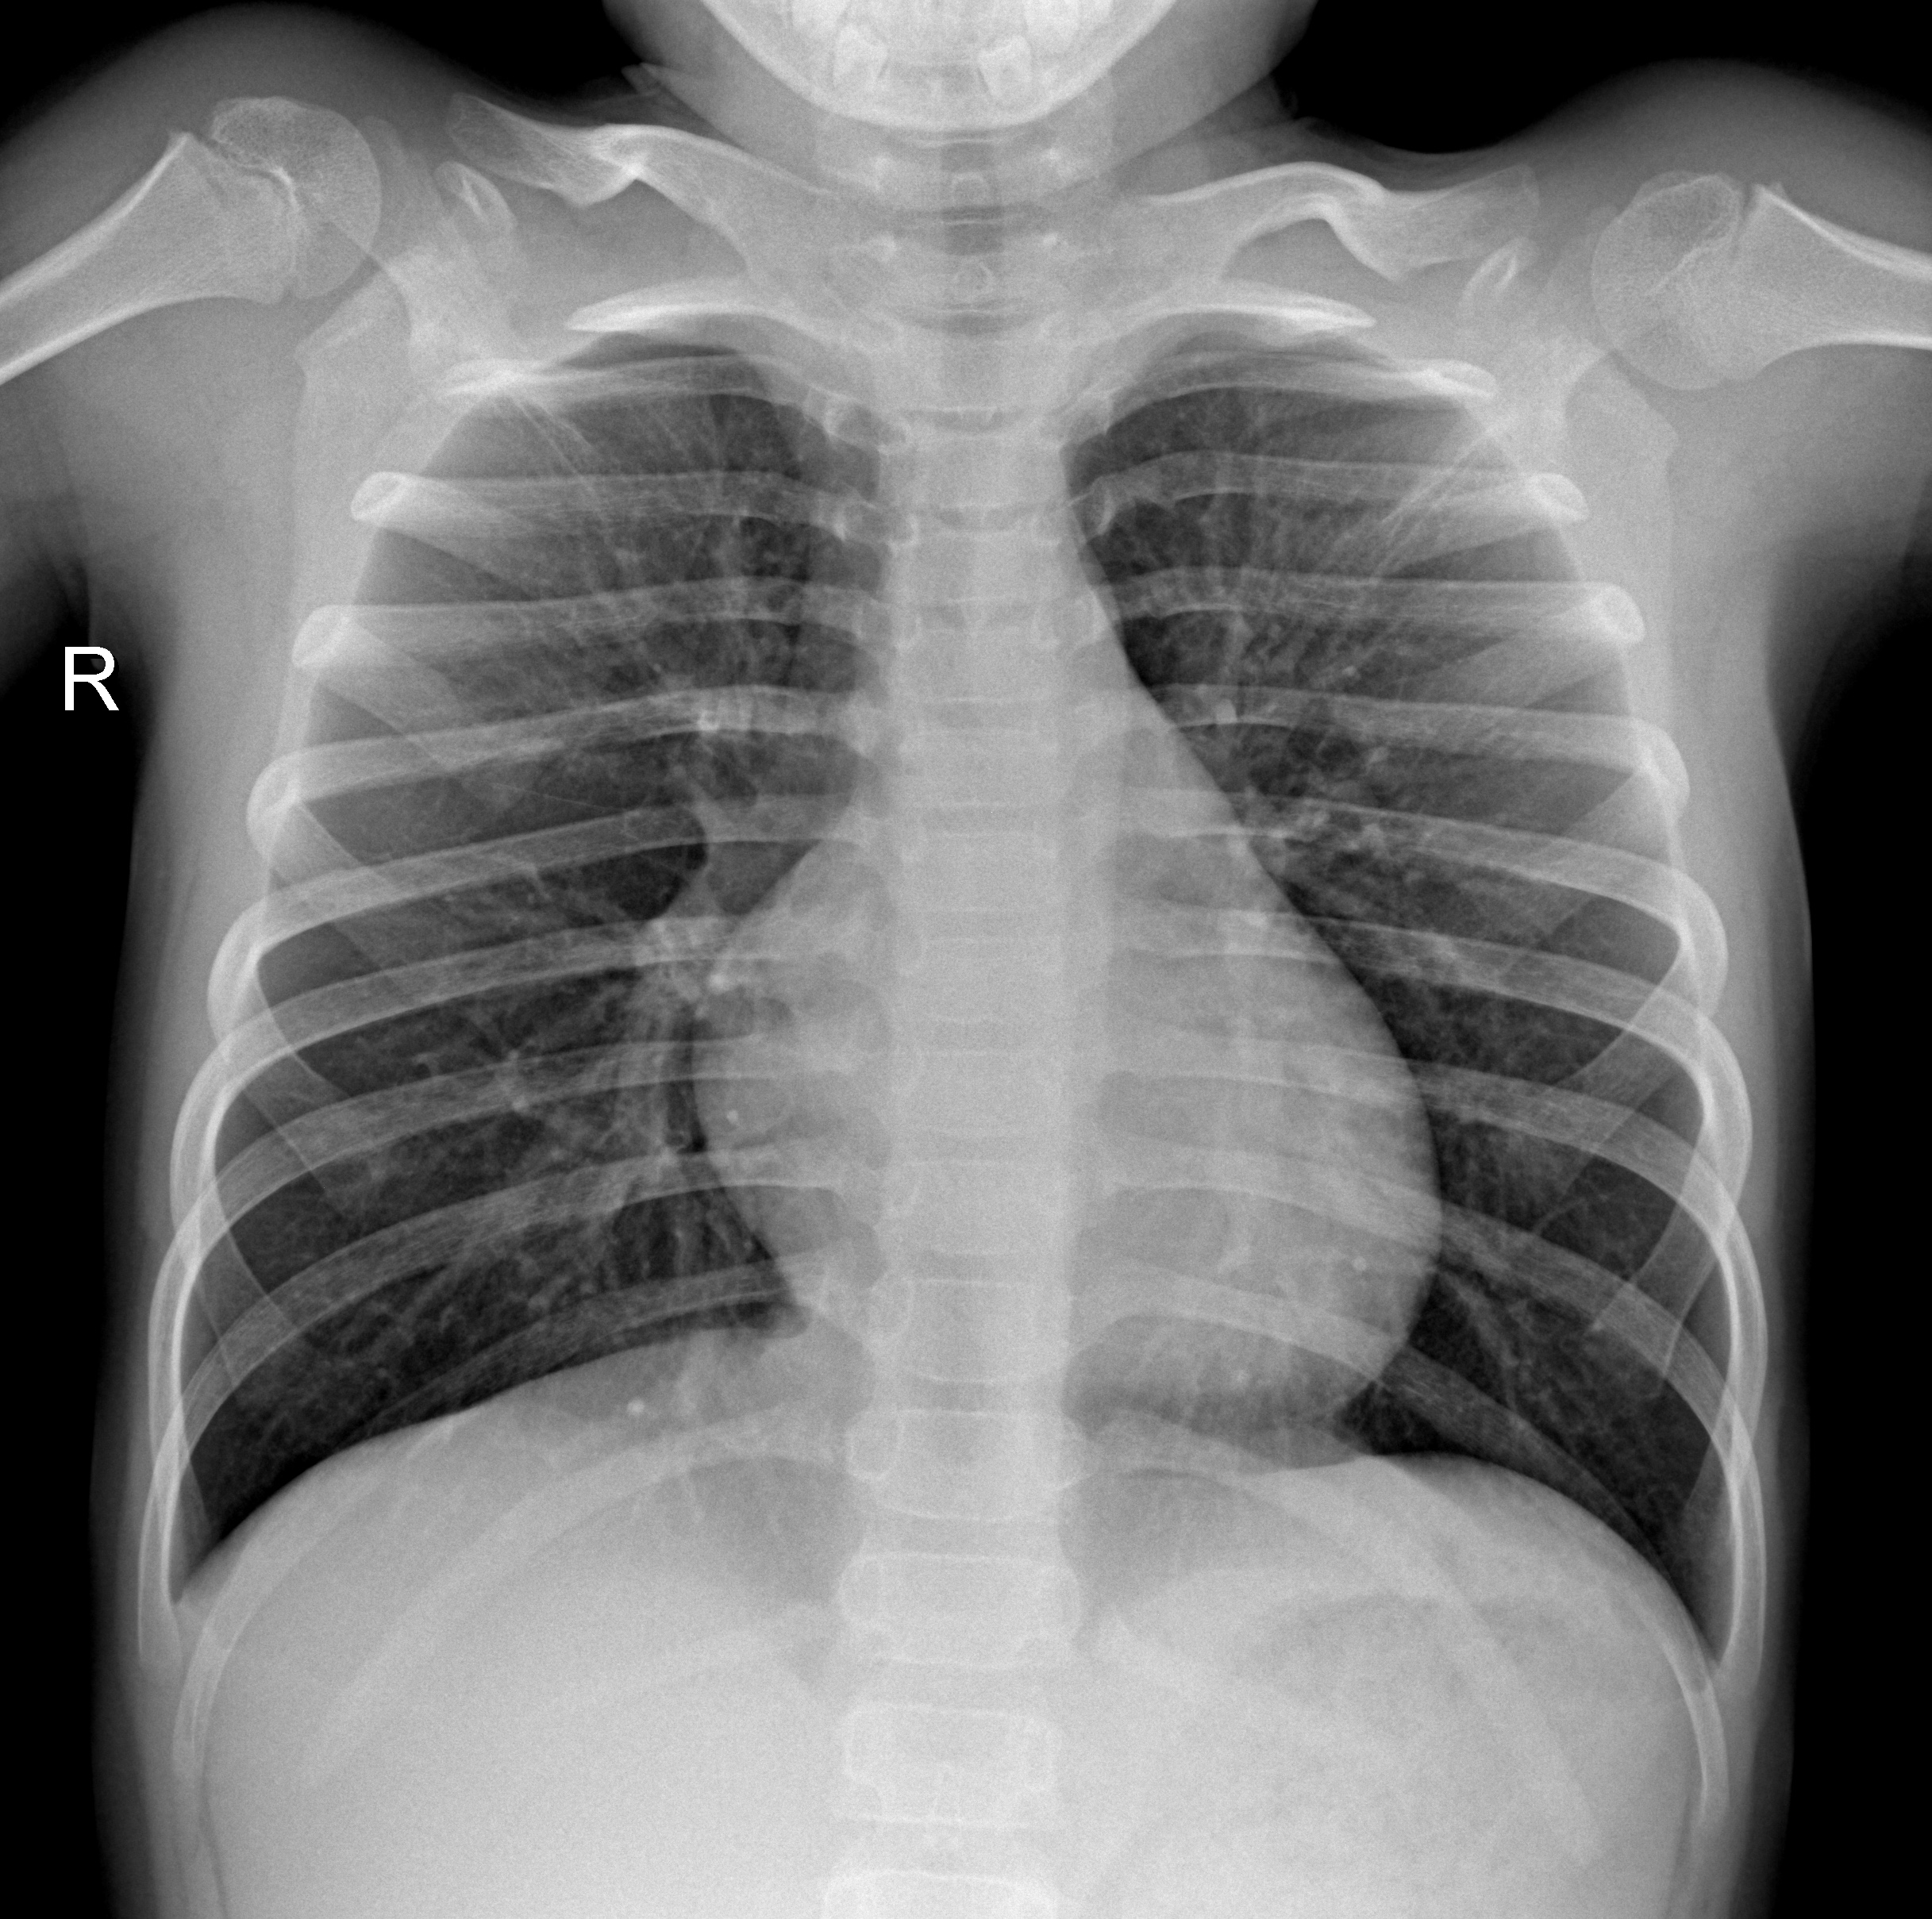
\includegraphics[width=0.4\textwidth]{Proposal/SampleNORMAL.jpeg}
    \caption{A sample image without pneumonia.\label{fig:SampleNORMAL}}
\end{figure}

\begin{figure}[H]
    \centering
    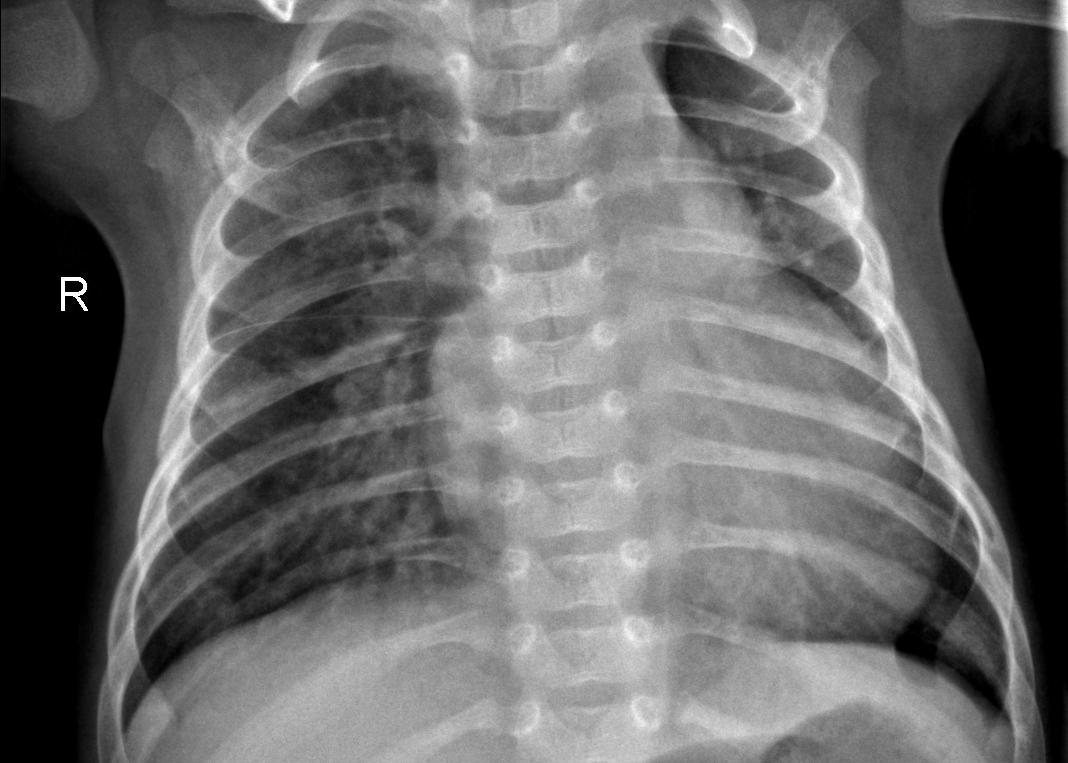
\includegraphics[width=0.4\textwidth]{Proposal/SamplePNEUMONIA.jpeg}
    \caption{A sample image with pneumonia.\label{fig:SamplePNEUMONIA}}
\end{figure}


\subsection{Additional observations}
The dataset has already been pre-emptively split into training and testing sets, which saves some preprocessing. 
However, the data itself is imperfect and will require further preprocessing before being used to train a model. 
Table \ref{tab:DatasetIssues} denotes the potential issues with the dataset's initial state.

\begin{longtable}{ | p{0.25\textwidth} | p{0.65\textwidth} | }
    \hline
    \cellcolor{blue!25} Issue & \cellcolor{blue!25} Explanation \\
    \hline
    Images are not all the same resolution. & The neural network's input layer will be fixed in size, meaning all input data must be the 
    same size or the network will be unable to process it. This can be addressed using Keras to automatically resize all images to a given 
    resolution.\\
    \hline
    Class imbalance & The training set contains 1,349 samples of patients without pneumonia, but 3,883 samples of patients with pneumonia.
    This will lead to the model favouring those with pneumonia rather than the underrepresented class of those without. This can be addressed 
    using the techniques discussed in Appendix A.\\
    \hline
    \caption{The issues with the dataset before any preprocessing.}\label{tab:DatasetIssues}
\end{longtable}

% ? 234 TestNorm, 390 TestPneu. 1349 TrainNorm, 3883 TrainPneu.


\section{Data science problem}
This dataset poses a clear data science problem pertaining to the classification of these images which will be addressed through the 
development of a neural network image classification model leveraging supervised learning. The ground truth is already present within  
% ? A "neural network" model? Be specific.
the dataset through its file structure, shown below:

\begin{verbatim}
    .
    `-- chest_xray/
        |-- test/
        |   |-- NORMAL/
        |   |   |-- NORMAL-4512-0001.jpeg
        |   |   |-- NORMAL-11419-0001.jpeg
        |   |   `-- ...234 more images
        |   `-- PNEUMONIA/
        |       |-- BACTERIA-40699-0001.jpeg
        |       |-- BACTERIA-227418-0001.jpeg
        |       `-- ...388 more images
        `-- train/
            |-- NORMAL/
            |   |-- NORMAL-28501-0001.jpeg
            |   |-- NORMAL-32326-0001.jpeg
            |   `-- ...1347 more images
            `-- PNEUMONIA/
                |-- BACTERIA-7422-0001.jpeg
                |-- BACTERIA-30629-0001.jpeg
                `-- ...3881 more images
\end{verbatim}

\noindent Files of the appropriate class are stored in the relevant subfolder. When this dataset is loaded, it will be possible to 
assign the relevant label to each image based on its subfolder of origin.

% "The aim is to develop a deep learning model to classify images into X classes."
% ? Describe the need for critical evaluation of the model.

% ! Footnote that the dataset contains multiple data science problems. I am only using "chest_xray", the 
% ! pneumonia identification problem.


\chapter{Related work}

% ! Added a ton of papers using this dataset to Zotero.
% ? You can use Litmaps to find more.

\section{Introduction}
"This section should demonstrate the main concepts
of related techniques that have been previously used to solve the problem."
\para What have other people done to solve it? How did they do it? 

% ! This is sectioned and divided exactly like your literature review.
% ! This section may be intensely difficult until the examples are uploaded for reference.

\section{Lit Review Topic 1}
% * Conventional machine learning methods (Random forest, SVM, etc)

\section{Lit Review Topic 2}


\section{Lit Review Topic 3}


% ?
% ! Example work has an extra chapter here titled "Concepts of Deep Learning" with 
% ! sections "Deep Neural Networks" and "Convolutional Neural Networks".
% ?

\chapter{Proposed model}
"This section should demonstrate the suitability of
the proposed solution in solving the data science problem"

% ? The model proposed here doesn't *need* to be the one you eventually use, but you should.


% ? When you submit your code, don't use your coloured comments like these.


\addcontentsline{toc}{chapter}{Bibliography}
\printbibliography

\end{document}